\section{Hardware}

Hardware (HW) omfatter systemet fra sensor til nettverksprotokollen som blir brukt i
bilsystemet. Hvilken HW
som trengs er da avhengig av noen faktorer:
\begin{itemize}
\item Tilgjengelige sensorer
\item Data format
\item Nødvendig dataprosessering
\item Utfordringer ved signaloverføring
\item Bruk av nettverksprotokoll
\end{itemize}

%hvilke sensorer som er tilgjengelige, hvilke data
%man får fra de ulike sensorene, hvilken dataprosessering som er nødvendig og
%utfordringer i forhold til signaloverføring og
%hvilken nettverksprotokoll som brukes. \\

\subsection{Definerende og begrensende faktorer}

En definerenede faktor for HW er måleteknikk. Det er da særlig krets
mellom eventuelt mikrokontroller (MCU) og sensor som vil variere. Ulike måleteknikker studeres
i seksjon \ref{subsec:sensorteknologier}. Måleteknikken setter også en begrensing på hva som er
mulig å måle og dermed hvilke tjenester systemet kan tilby. \\

I bilindustrien er CAN den rådende nettverksprotokollen (sjekke med ref). Man
kan argumentere for at man på grunnlag av dette burde integrere nye systemer på
det eksisterende nettverket. Uansett hvilket nettverk det skal kommuniseres over
vil det stille krav til HW. En ny enhet bør ha riktig nettverksgrensesnitt
og må kunne kommunisere på riktig protokoll. \\

\subsection{Sensorteknologier}
\label{subsec:sensorteknologier}

% TODO: Teknologi, utfordringer, løsninger

(Denne er seksjonen er tildels uferdig). \\

Det er mange fysiske prinsipper som kan måles for å detektere en løs hjulmutter.
Det er derfor viktig å undersøke hvilke sensorteknologier som er tilgjengelig og
hvilke fordeler disse drar med seg. \\

Tre ulike fysiske prinsipper som kan brukes er strekk, trykk og vibrasjon. \\

\subsection{Vibrasjonsmåling}

Vibrasjonsmåling kan bli gjort med teknologier som et akselerometer eller ved
pizoelektriske microfoner. Slike sensorer vil kunne gi et signal som inneholder
ulike frekvenstyper som kan analyseres. Slik kan man gjenkjenne mønstre i
frekvensbåndet som indikerer eksempevis en løs mutter. For å analysere dette signalet må det
samples med en Analog-til-Digital Converter (ADC). Dersom signalet er svakt må det også forsterkes gjennom en
forsterker krets. For å hente ut informasjon av signalet må en algoritme undersøke
frekvensoppbyggingen av signalet. Dette kan bli gjort i HW med en Digital Signal Processor (DSP), men kan
også gjøres i software (SW) ved at det sendes en signalprøve fra HW til controlsystemet. Å
bruke en DSP kompliserer HW og effektforbruk og kost øker. Analyserer man
signalet i SW slipper man disse konsekvensene og det blir lettere å oppdatere
algoritmen dersom det er nødvendig. \\

Kommunikasjon skjer ved å sende CAN pakker på et eksisterende nettverk. Pakkene
inneholder målinger tatt periodisk med et gitt samplingsvindu. Man må da se
nærmere på hvor stor dette vinduet bør være samt hvor ofte målingen må tas. Det
er kanskje nødvendig med analog filtrering av signalet (før ADC). \\

Tanken er å ha sensoren på akslingen mellom to hjul. For å skille mellom hvilket
hjul som har løse muttere, så kan det være en løsning å bruke en sensor ved vært
hjul. Da er to mulig algoritmer å måle amplitudeforskjell eller
tidsforsinkelse. Dette burde være mulig å få til med en MCU, men kan være det
blir nødvendig med en DSP for raskere prosessering av signalene. \\

MCUen sender pakkene med en ID slik at man kan skille mellom ulike akslinger. \\

\subsection{Strekklapper/Trykklapper}

Tanken er å legge strekklapper inni eller på utsiden av boltene eller
trykklapper mellom bolt og nav. Strekklappene
må/kan/bør legges i en krets (Wheatstone feks) for å kunne gi ut et målbart
spenningsnivå. For å oppnå et målbart spenningsnivå må man mest sannsynlig
forsterke signalet gjennom en In Amp. Denne analoge målingen krever mye lavere sampling end ved
vibrasjonsmålinger da det trengs kortere signalprøver.
Man kan få problemer med at signalet fra strekklappen må gjennom en slepering.
Dette kan by på utfordringer med tanke på implementasjon og støy.
Man må også ha en sensor per bolt. Dette fører til mer HW. En måte å redusere
mengden HW på kan være å MUX'e signalene fra hver sensor til MCU. Det er mulig å lage
en krets hvor man benytter seg av tidskonstanten i en RC-krets (dette må du
undersøke litt). Overføring av
signaler fra nav til aksling kan også skje ved induksjon (dette må du undersøke
litt mer). For å koble til flere
enheter på et CAN nettverk så kan man benytte seg av J1939 som fordelere ID på
nettverket (dette må du undersøke litt mer). \\

\begin{figure}[H]
\subfigure[]{
	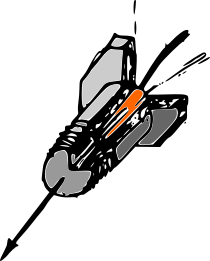
\includegraphics[width=0.4 \textwidth]{images/Straingage_vector.png}
	\label{fig:Strekklapp_vector}
	}
\hfill
\subfigure[]{
	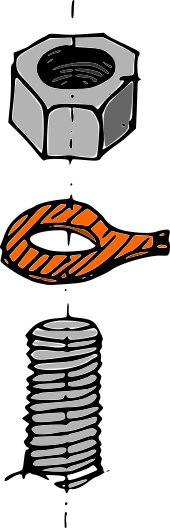
\includegraphics[width=0.2 \textwidth]{images/trykklapp_vector.png}
	\label{fig:Trykklapp_vector}
	}
\caption{\protect{\ref{fig:Strekklapp_vector}} Strekklapp i bolt (orange), \protect{\ref{fig:Trykklapp_vector}} Trykklapp (orange) mellom bolt og mutter.}
\end{figure}

\subsection{Utfordringer}

Problemet med å måle vibrasjoner er at en sampleprøve av et signal innenfor et gitt tidsrom kan bli veldig stor. Som
et resultat at de store sampleprøvene kan det oppstå båndbreddeproblemer på CAN-bussen. Grunnen til dette
er at samplingsfrekvensen man sampler signalet med må være
minst dobbelt så høy som frekvensen av signalet, if ølge Nyquist–Shannon sampling theorem \cite{nyquist}. Høyere
samplingsrate gir bedre signalrepresentasjon, og en god
representasjon av signalet kan være viktig for en eventuell analysealgoritme.

Dersom analysealgoritmen kjøres på en DSP slipper CAN-bussen og overbelastes av store datamengder.
Algoritmen ligger ikke da i det sentrale systemet og det kan bli vanskeligere å forbedre algoritmen ved hjelp av AI.
